\documentclass[10 pt,usenames,dvipsnames, oneside]{article}
\usepackage{../../../modelo-ensino-medio}



\begin{document}

\begin{center}
  \begin{minipage}[l]{3cm}

\includegraphics[width=2cm]{logo}    
\end{minipage}\hfill
\begin{minipage}[r]{.8\textwidth}
 {\Large \scshape Atividade: Medindo ângulos centrais em nosso planeta}  
\end{minipage}
\end{center}
\vspace{.2cm}

\ifdefined\prof
%Habilidades da BNCC
% \begin{objetivos}
% \item 
% \end{objetivos}

%Caixa do Para o Professor
\begin{goals}
%Objetivos específicos
\begin{enumerate}
\item Medir empiricamente arcos e ângulos
\item Usar ferramentas tecnológicas no trabalho com arcos e ângulo
\end{enumerate}


\end{goals}

\bigskip
\begin{center}
{\large \scshape Atividade}
\end{center}
\fi

Um dos resultados mais fascinantes que já existiram na História da Matemática é decorrente do experimento realizado pelo matemático e astrônomo grego Eratóstenes. Estudando o comportamento das sombras de varetas nas cidades Alexandria e Syene (Assuã, nos dias atuais) ao meio dia, ele não só conseguiu perceber que a superfície da Terra não era plana como conseguiu calcular, com uma precisão surpreendente, o comprimento de uma volta completa ao redor da Terra!

Eratóstenes sabia que a distância entre as cidades de Alexandria e Syene era aproximadamente igual a $800$ km. Percebeu também que ao meio dia, o sol estava a pino em Syene de forma que nesse horário, podia-se ver o sol completamente refletido no interior do poço. Além disso, às $12$ h, nenhuma sombra era formada pelas colunas daquela cidade. O mesmo não ocorria em Alexandria: ao meio dia, uma vareta colocada de pé no chão apresentava uma sombra substancial e com ela, Eratóstenes conseguiu provar que o arco sobre a superfície da Terra, que compreende as cidades de Alexandria e Assuã media cerca de $\frac{\pi}{25}\rad$ ($7{,}2$ graus) e que corresponde ao ângulo central $\hat{A}$ da \hyperref[zenite]{figura \ref{zenite}}:

\begin{figure}[H]
\centering

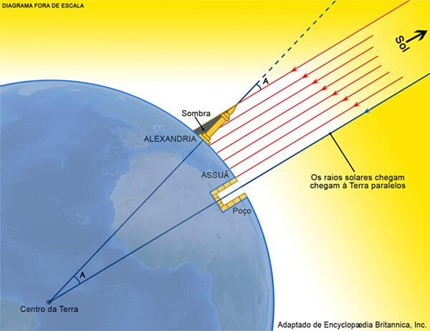
\includegraphics[width=.65\linewidth]{trigonometricas42}
\caption{Costa, J. R. V. Eratóstenes e a circunferência da Terra. \href{https://www.zenite.nu/eratostenes-e-a-circunferencia-da-terra/}{Astronomia no Zênite}, jul 2000.}
\label{zenite}
\end{figure}

Eratóstenes utilizou a seguinte regra de três para calcular o comprimento de uma volta completa ao redor da Terra:


\begin{equation*}
\begin{array}{ccc}
\frac{\pi}{25} \rad & \adjustbox{valign=c}{\tikz \draw (0,0) -- (1.5,0);} & 800 \text{ km} \\
2\pi\rad & \adjustbox{valign=c}{\tikz \draw (0,0) -- (1.5,0);} & C 
\end{array}
\end{equation*}

Resolvendo a regra de três, obtemos $C = 40.000$ km. Utilizando instrumentos tecnológicos muito mais avançados dos quais dispunha Eratóstenes, hoje se sabe que o comprimento de uma volta completa na Terra é de $40.072$ km, ou seja, o erro de cálculo do matemático grego foi de menos de $100$ km! O vídeo a seguir, apresenta parte de um episódio famosa série Cosmos, e narra com mais detalhes a ideia do experimento de Eratóstenes.

\begin{figure}[H]
\centering

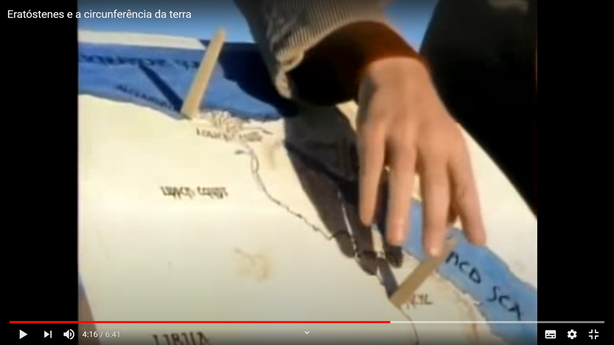
\includegraphics[width=.5\linewidth]{trigonometricas43}

\caption{Acesse pelo link: \url{https://www.youtube.com/watch?v=fu9Z7YuXLVE}}
\end{figure}

Vamos utilizar o raciocínio de Eratóstenes, com o auxílio do Google Earth para medir arcos em graus e radianos, limitados por duas cidades brasileiras! Baixe e instale no seu smartphone o aplicativo Google Earth.


\begin{figure}[H]
\centering

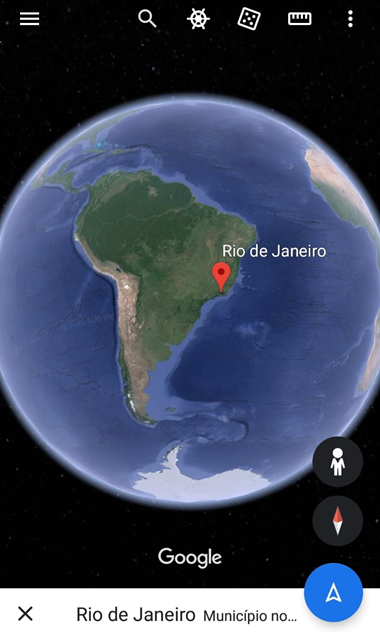
\includegraphics[height=.3\textheight]{trigonometricas44}
\end{figure}

\begin{enumerate}
\item Use a ferramenta medir para encontrar uma aproximação para distância, ao longo do globo terrestre, entre as capitais Rio de Janeiro e Belo Horizonte.
\item Usando o fato que uma volta completa na Terra tem $40.072$ km, determine a medida aproximada do valor do arco (em radianos) sobre a superfície da Terra que liga as duas capitais do item \titem{a)}.
\item Reproduza os itens \titem{a)} e \titem{b)} para a cidade onde você mora e qualquer outra cidade de sua escolha no Brasil.
\end{enumerate}

\ifdefined\prof
\begin{solucao}

\begin{enumerate}
\item Aproximadamente $340$ km.
\item Aproximadamente $0{,}053\rad$.
\item Valores dependerão das escolhas dos alunos.
\end{enumerate}

\end{solucao}
\fi

\end{document}